\documentclass[pdf, unicode, 9pt, notheorems, handout]{beamer}

%\mode<handout> {
%    \usepackage{pgfpages}
%    \setbeameroption{show notes}
%    \pgfpagesuselayout{2 on 1}[a4paper, border shrink=5mm]
%    \setbeamercolor{note page}{bg=white}
%    \setbeamercolor{note title}{bg=gray!10}
%    \setbeamercolor{note date}{fg=gray!10}
%}

\usepackage[utf8]{inputenc}
\usepackage[T2A]{fontenc}
\usepackage[russian, english]{babel}
\usepackage{ragged2e}
%\usepackage{t-angles}
%\usepackage{slashbox}
\usepackage{hhline}
\usepackage{beamerthemesplit}

%new calligraphic font for subspaces 
\usepackage{euscript}
\newcommand{\cA}{\EuScript{A}}
\newcommand{\cB}{\EuScript{B}}
\newcommand{\cC}{\EuScript{C}}
\newcommand{\cD}{\EuScript{D}}
\newcommand{\cE}{\EuScript{E}}
\newcommand{\cF}{\EuScript{F}}
\newcommand{\cG}{\EuScript{G}}
\newcommand{\cH}{\EuScript{H}}
\newcommand{\cI}{\EuScript{I}}
\newcommand{\cJ}{\EuScript{J}}
\newcommand{\cK}{\EuScript{K}}
\newcommand{\cL}{\EuScript{L}}
\newcommand{\cM}{\EuScript{M}}
\newcommand{\cN}{\EuScript{N}}
\newcommand{\cO}{\EuScript{O}}
\newcommand{\cP}{\EuScript{P}}
\newcommand{\cQ}{\EuScript{Q}}
\newcommand{\cR}{\EuScript{R}}
\newcommand{\cS}{\EuScript{S}}
\newcommand{\cT}{\EuScript{T}}
\newcommand{\cU}{\EuScript{U}}
\newcommand{\cV}{\EuScript{V}}
\newcommand{\cW}{\EuScript{W}}
\newcommand{\cX}{\EuScript{X}}
\newcommand{\cY}{\EuScript{Y}}
\newcommand{\cZ}{\EuScript{Z}}

%font for text indices like transposition X^\mathrm{T}
\newcommand{\rmA}{\mathrm{A}}
\newcommand{\rmB}{\mathrm{B}}
\newcommand{\rmC}{\mathrm{C}}
\newcommand{\rmD}{\mathrm{D}}
\newcommand{\rmE}{\mathrm{E}}
\newcommand{\rmF}{\mathrm{F}}
\newcommand{\rmG}{\mathrm{G}}
\newcommand{\rmH}{\mathrm{H}}
\newcommand{\rmI}{\mathrm{I}}
\newcommand{\rmJ}{\mathrm{J}}
\newcommand{\rmK}{\mathrm{K}}
\newcommand{\rmL}{\mathrm{L}}
\newcommand{\rmM}{\mathrm{M}}
\newcommand{\rmN}{\mathrm{N}}
\newcommand{\rmO}{\mathrm{O}}
\newcommand{\rmP}{\mathrm{P}}
\newcommand{\rmQ}{\mathrm{Q}}
\newcommand{\rmR}{\mathrm{R}}
\newcommand{\rmS}{\mathrm{S}}
\newcommand{\rmT}{\mathrm{T}}
\newcommand{\rmU}{\mathrm{U}}
\newcommand{\rmV}{\mathrm{V}}
\newcommand{\rmW}{\mathrm{W}}
\newcommand{\rmX}{\mathrm{X}}
\newcommand{\rmY}{\mathrm{Y}}
\newcommand{\rmZ}{\mathrm{Z}}

%tt font for time series
\newcommand{\tA}{\mathsf{A}}
\newcommand{\tB}{\mathsf{B}}
\newcommand{\tC}{\mathsf{C}}
\newcommand{\tD}{\mathsf{D}}
\newcommand{\tE}{\mathsf{E}}
\newcommand{\tF}{\mathsf{F}}
\newcommand{\tG}{\mathsf{G}}
\newcommand{\tH}{\mathsf{H}}
\newcommand{\tI}{\mathsf{I}}
\newcommand{\tJ}{\mathsf{J}}
\newcommand{\tK}{\mathsf{K}}
\newcommand{\tL}{\mathsf{L}}
\newcommand{\tM}{\mathsf{M}}
\newcommand{\tN}{\mathsf{N}}
\newcommand{\tO}{\mathsf{O}}
\newcommand{\tP}{\mathsf{P}}
\newcommand{\tQ}{\mathsf{Q}}
\newcommand{\tR}{\mathsf{R}}
\newcommand{\tS}{\mathsf{S}}
\newcommand{\tT}{\mathsf{T}}
\newcommand{\tU}{\mathsf{U}}
\newcommand{\tV}{\mathsf{V}}
\newcommand{\tW}{\mathsf{W}}
\newcommand{\tX}{\mathsf{X}}
\newcommand{\tY}{\mathsf{Y}}
\newcommand{\tZ}{\mathsf{Z}}

%bf font for matrices
\newcommand{\bfA}{\mathbf{A}}
\newcommand{\bfB}{\mathbf{B}}
\newcommand{\bfC}{\mathbf{C}}
\newcommand{\bfD}{\mathbf{D}}
\newcommand{\bfE}{\mathbf{E}}
\newcommand{\bfF}{\mathbf{F}}
\newcommand{\bfG}{\mathbf{G}}
\newcommand{\bfH}{\mathbf{H}}
\newcommand{\bfI}{\mathbf{I}}
\newcommand{\bfJ}{\mathbf{J}}
\newcommand{\bfK}{\mathbf{K}}
\newcommand{\bfL}{\mathbf{L}}
\newcommand{\bfM}{\mathbf{M}}
\newcommand{\bfN}{\mathbf{N}}
\newcommand{\bfO}{\mathbf{O}}
\newcommand{\bfP}{\mathbf{P}}
\newcommand{\bfQ}{\mathbf{Q}}
\newcommand{\bfR}{\mathbf{R}}
\newcommand{\bfS}{\mathbf{S}}
\newcommand{\bfT}{\mathbf{T}}
\newcommand{\bfU}{\mathbf{U}}
\newcommand{\bfV}{\mathbf{V}}
\newcommand{\bfW}{\mathbf{W}}
\newcommand{\bfX}{\mathbf{X}}
\newcommand{\bfY}{\mathbf{Y}}
\newcommand{\bfZ}{\mathbf{Z}}

%bb font for standard spaces and expectation
\newcommand{\bbA}{\mathbb{A}}
\newcommand{\bbB}{\mathbb{B}}
\newcommand{\bbC}{\mathbb{C}}
\newcommand{\bbD}{\mathbb{D}}
\newcommand{\bbE}{\mathbb{E}}
\newcommand{\bbF}{\mathbb{F}}
\newcommand{\bbG}{\mathbb{G}}
\newcommand{\bbH}{\mathbb{H}}
\newcommand{\bbI}{\mathbb{I}}
\newcommand{\bbJ}{\mathbb{J}}
\newcommand{\bbK}{\mathbb{K}}
\newcommand{\bbL}{\mathbb{L}}
\newcommand{\bbM}{\mathbb{M}}
\newcommand{\bbN}{\mathbb{N}}
\newcommand{\bbO}{\mathbb{O}}
\newcommand{\bbP}{\mathbb{P}}
\newcommand{\bbQ}{\mathbb{Q}}
\newcommand{\bbR}{\mathbb{R}}
\newcommand{\bbS}{\mathbb{S}}
\newcommand{\bbT}{\mathbb{T}}
\newcommand{\bbU}{\mathbb{U}}
\newcommand{\bbV}{\mathbb{V}}
\newcommand{\bbW}{\mathbb{W}}
\newcommand{\bbX}{\mathbb{X}}
\newcommand{\bbY}{\mathbb{Y}}
\newcommand{\bbZ}{\mathbb{Z}}

%got font for any case
\newcommand{\gA}{\mathfrak{A}}
\newcommand{\gB}{\mathfrak{B}}
\newcommand{\gC}{\mathfrak{C}}
\newcommand{\gD}{\mathfrak{D}}
\newcommand{\gE}{\mathfrak{E}}
\newcommand{\gF}{\mathfrak{F}}
\newcommand{\gG}{\mathfrak{G}}
\newcommand{\gH}{\mathfrak{H}}
\newcommand{\gI}{\mathfrak{I}}
\newcommand{\gJ}{\mathfrak{J}}
\newcommand{\gK}{\mathfrak{K}}
\newcommand{\gL}{\mathfrak{L}}
\newcommand{\gM}{\mathfrak{M}}
\newcommand{\gN}{\mathfrak{N}}
\newcommand{\gO}{\mathfrak{O}}
\newcommand{\gP}{\mathfrak{P}}
\newcommand{\gQ}{\mathfrak{Q}}
\newcommand{\gR}{\mathfrak{R}}
\newcommand{\gS}{\mathfrak{S}}
\newcommand{\gT}{\mathfrak{T}}
\newcommand{\gU}{\mathfrak{U}}
\newcommand{\gV}{\mathfrak{V}}
\newcommand{\gW}{\mathfrak{W}}
\newcommand{\gX}{\mathfrak{X}}
\newcommand{\gY}{\mathfrak{Y}}
\newcommand{\gZ}{\mathfrak{Z}}

%old calligraphic font
\newcommand{\calA}{\mathcal{A}}
\newcommand{\calB}{\mathcal{B}}
\newcommand{\calC}{\mathcal{C}}
\newcommand{\calD}{\mathcal{D}}
\newcommand{\calE}{\mathcal{E}}
\newcommand{\calF}{\mathcal{F}}
\newcommand{\calG}{\mathcal{G}}
\newcommand{\calH}{\mathcal{H}}
\newcommand{\calI}{\mathcal{I}}
\newcommand{\calJ}{\mathcal{J}}
\newcommand{\calK}{\mathcal{K}}
\newcommand{\calL}{\mathcal{L}}
\newcommand{\calM}{\mathcal{M}}
\newcommand{\calN}{\mathcal{N}}
\newcommand{\calO}{\mathcal{O}}
\newcommand{\calP}{\mathcal{P}}
\newcommand{\calQ}{\mathcal{Q}}
\newcommand{\calR}{\mathcal{R}}
\newcommand{\calS}{\mathcal{S}}
\newcommand{\calT}{\mathcal{T}}
\newcommand{\calU}{\mathcal{U}}
\newcommand{\calV}{\mathcal{V}}
\newcommand{\calW}{\mathcal{W}}
\newcommand{\calX}{\mathcal{X}}
\newcommand{\calY}{\mathcal{Y}}
\newcommand{\calZ}{\mathcal{Z}}


\usefonttheme[onlymath]{serif}
\usetheme[numbers, totalnumbers, compress, nologo]{Statmod}
\setbeamerfont{institute}{size=\normalsize}
\setbeamertemplate{navigation symbols}{}

\setbeamercolor{bluetext_color}{fg=blue}
\newcommand{\bluetext}[1]{{\usebeamercolor[fg]{bluetext_color}#1}}

\newtheorem{theorem}{Теорема}
\newtheorem{statement}{Утверждение}
\newtheorem{definition}{Определение}

\title{Тензорный анализ сингулярного спектра}

\author{Хромов Никита Андреевич, гр.20.Б04-мм}

\institute[Санкт-Петербургский Государственный Университет]{
    Санкт-Петербургский государственный университет\\
    Прикладная математика и информатика\\
    Вычислительная стохастика и статистические модели\\
    \vspace{0.7cm}
    Научный руководитель:  д.ф.-м.н. Голяндина Н.Э.  \\
    Рецензент: к.ф.-м.н. Усевич К.Д.}

\date{Санкт-Петербург,\\ \number\year}

\begin{document}
    
    \begin{frame}[plain, noframenumbering]
        \titlepage
    \end{frame}
    
    
    %\section{Короткая тема}
    %\subsection{Общие слова}
    
    
    \section{Введение}\label{sec:intro}
    \begin{frame}{Постановка задачи}
        $\tX_p = \left(x_1^{(p)}, x_2^{(p)}, \ldots, x_N^{(p)}\right)$, $x_i \in \bbR$ --- одномерный 
        временной ряд\\         
        $\tX = (\tX^{(1)} : \tX^{(2)} : \ldots : \tX^{(P)})$ --- многомерный временной ряд\\ \vspace{0.2cm} 
        $\tX = \tT + \tP + \tE$ \\ 
        $\tT$ --- медленно меняющаяся компонента (тренд)\\ 
        $\tP$ --- периодическая компонента (сезонность)\\ 
        $\tE$ --- случайная компонента (шум)\\ 
        \vspace{0.2cm}
        
        \bluetext{Возможные задачи:}
        \begin{enumerate}
            \item Выделение сигнала из ряда: нахождение $\tS = \tT + \tP$
            \item Разделение сигнала: нахождение компонент $\tT$ и $\tP$
        \end{enumerate}
        \vspace{0.2cm}
        
        Возможный метод решения: Singular Spectrum Analysis (\bluetext{SSA})
        
        [Golyandina, Nekrutkin et al. (2001)],\\
        и его многомерное расширение Multivariate SSA (\bluetext{MSSA})
        
        [Голяндина, Степанов (2005)]
        
%        , Analysis of time series structure: SSA and related trchniques)\\
        \vspace{0.3cm}
        
        {\color{red} Цель:} реализация тензорных расширений методов SSA и MSSA, исследование их свойств с точки
        зрения точности выделения сигнала и разделения компонент, сравнение расширений с базовыми методами.
    \end{frame}
    
    
    \section{Известные результаты}\label{sec:known-results}
    \begin{frame}{Схема методов SSA и MSSA}
        $\tX = \sum_{k=1}^{m}\tX_k + \tE$ --- (многомерный) временной ряд,\\
%        $L$ --- длина окна (параметр),\\
%        $K = N - L + 1 \geqslant L$.\\
        \vspace{0.2cm}
        
        \bluetext{Параметры алгоритма:} $L < N$ --- длина окна, $K=N-L+1$,\\
        $R$ --- число элементов разложения, относимых к сигналу,\\
        $\gI_1,\ldots, \gI_m \subseteq \{1, 2, \ldots, R\}$, $\gI_i \cap \gI_j = \varnothing$ --- наборы индексов,
        относимых к компонентам сигнала.
        \vspace{0.2cm}
        
        \bluetext{Схема алгоритма MSSA для разделения компонент сигнала}
        \begin{enumerate}
            \item \bluetext{Вложение}
            $\tX \overset{L}{\longmapsto} \bfX = \left[\bfX^{(1)} : \bfX^{(2)} : \ldots : \bfX^{(P)}\right] \in \bbR^{L\times{}KP}$,
            $\bfX^{(p)} =  \left[X_1^{(p)} : X_2^{(p)} : \ldots : X_K^{(p)}\right] \in \bbR^{L \times K}$,\\
            $X_i^{(p)} = (x_i^{(p)}, x_{i+1}^{(p)}, \ldots, x_{i+L-1}^{(p)})^{\rmT}$\\
            
            \item \bluetext{Разложение} $\bfX = \sum_{j=1}^{d} \sqrt{\lambda_j}
            U_j V_j^{\rmT}$, $\quad d \leqslant \min(L, KP)$
            \item \bluetext{Группировка}  $\widetilde{\bfX}_k = \sum_{j\in \gI_k} \sqrt{\lambda_j}
            U_j V_j^{\rmT}$, $\quad R\leqslant d$\\
            $\widetilde{\bfX}_k = \left[\widetilde{\bfX}_k^{(1)} : \widetilde{\bfX}_k^{(2)} : \ldots :
            \widetilde{\bfX}_k^{(P)}\right]$
            \item \bluetext{Восстановление} усреднение $\widetilde{\bfX}_k^{(p)}$ вдоль побочных
            диагоналей
%             $\tilde{x}_n^{(p)} = \operatorname{mean}\left\{\left(\widetilde{\bfX}_k^{(p)}\right)_{ij}
%            \middle| i + j - 1 = n\right\}$
        \end{enumerate}
        \vspace{0.2cm}
        
        \bluetext{Результат алгоритма} $\widetilde{\tX}_k$
%         = (\tilde{s}_1, \tilde{s}_2, \ldots, \tilde{s}_N)$ 
         --- оценки компонент $\tX_k$
    \end{frame}
    
    \begin{frame}{Разделимость и ранги рядов}
        \begin{itemize}
            \item \bluetext{Разделимость:} пусть $\tX = \tX_1 + \tX_2$
            \[
            \bfX = \sideset{}{_{j=1}^d}\sum\nolimits \sqrt{\lambda_j} U_j V_j^{\rmT} \stackrel{\displaystyle ?}{=}
            \overbrace{\sideset{}{_{j\in \gI_1}}\sum\nolimits \sqrt{\lambda_j} U_j V_j^{\rmT}}^{\bfX_1} +
            \overbrace{\sideset{}{_{j\in \gI_2}}\sum\nolimits \sqrt{\lambda_j} U_j V_j^{\rmT}}^{\bfX_2}
            \]
            \begin{definition}
                Траекторное пространство 
                $\Lambda^{(1,L)}(\tX)$ --- пространство столбцов матрицы $\bfX$, построенной по длине окна $L$,
                $\Lambda^{(2,K)}(\tX)$ --- пространство её строк.
            \end{definition}
            \vspace{0.1cm}
            $\tX_1$ и $\tX_2$ $L$-разделимы $\iff \Lambda^{(1,L)}(\tX_1) \perp \Lambda^{(1,L)}(\tX_2)$ и
            $\Lambda^{(2,K)}(\tX_1) \perp \Lambda^{(2,K)}(\tX_2)$\\ \vspace{0.1cm}
            \item \bluetext{Ранг ряда:} выбор параметра $R$?
            \begin{definition}
                $\tX$ имеет ранг $d$ $(\operatorname{rank}\tX = d)$, если $\forall L$: $d\leqslant \min(L, N-L+1)$\\
                $\operatorname{dim}\Lambda^{(L)}(\tX)=d$
            \end{definition}
            Рекомендуемый выбор $R= \operatorname{rank}\tX$
        \end{itemize}
    \end{frame}
    
    \begin{frame}{Переход к тензорам}
        \begin{table}
            \hspace*{-0.38cm}
            \begin{tabular}{rlllll}
                \bluetext{Базовый алгоритм:} & ряд $\tX$ & $\Rightarrow$ & матрица $\mathbf{X}$ & $\Rightarrow$ & SVD $\mathbf{X}$ \\
                \hfill &&&&&\\
                \bluetext{Тензорный алгоритм:} & ряд $\tX$ & $\Rightarrow$ & тензор $\mathcal{X} $ & $\Rightarrow$ &
                \hspace*{-0.3cm} \begin{tabular}{l}
                    тензорное  \\
                    разложение
                \end{tabular} $\mathcal{X}$
            \end{tabular}
        \end{table}
        
        \vspace{0.4cm}
        Тензорные разложения, расширяющие SVD [Sidiropoulos et al. (2016)]:
        \begin{itemize}
            \item Higher-order singular value decomposition (\bluetext{HOSVD})
            \item Canonical polyadic decomposition (CPD)
            \item ($L_r, L_r, 1)$-decomposition
        \end{itemize}
        
        \vspace{0.5cm}
        
        Тензорный переход с HOSVD для оценки параметров сигнала особого вида:
        [Papy et al. (2005)]
    \end{frame}
    
        
    \section{Higher-Order SSA}\label{sec:ho-ssa}
    \begin{frame}{Траекторный тензор}
        \centering
        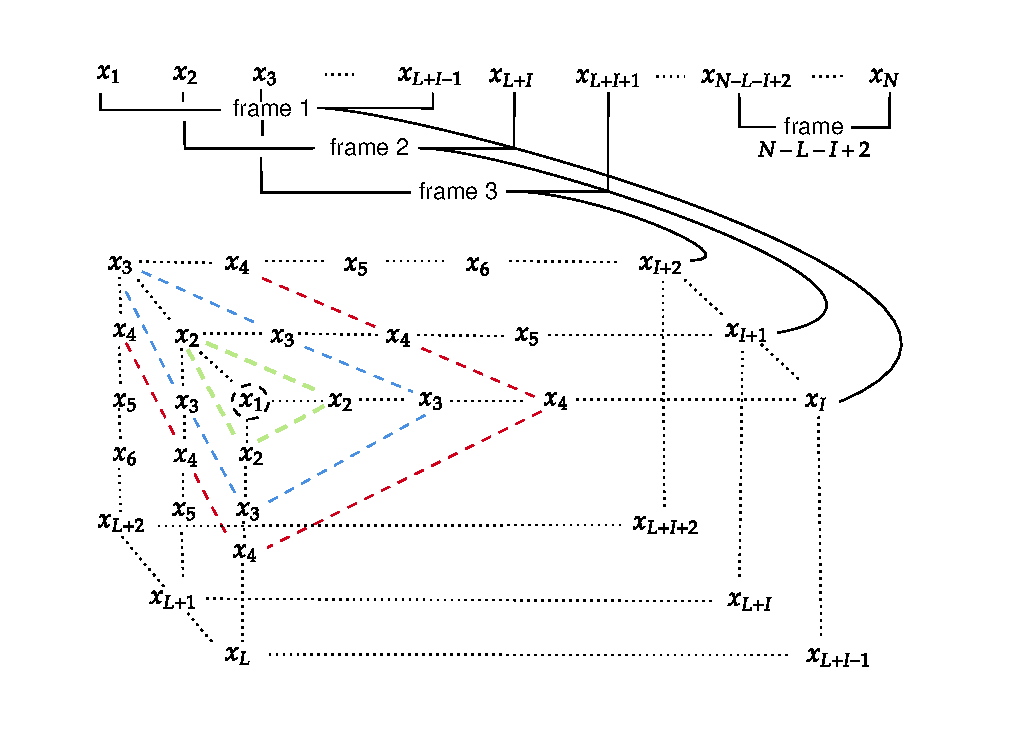
\includegraphics[width = \textwidth]{./img/tens-injection-wide}\\{}
        \vspace{-0.4cm}
        
        $I, L$ --- параметры длины окна
    \end{frame}
    
    \begin{frame}{Higher-Order SSA}
        $\tX = \sum_{k=1}^{m}\tX_k + \tE$ --- одномерный временной ряд\\ \vspace{0.2cm}
        
        \bluetext{Параметры алгоритма:} $I,L < N$ --- длины окна, $I + L < N + 1$,  $J=N-I-L+2$;
        $R$, $\gI_1,\ldots, \gI_m$ --- как в SSA
        \vspace{0.3cm}
        
        \bluetext{Схема алгоритма HO-SSA для разделения компонент сигнала}
        \begin{enumerate}
            \item \bluetext{Вложение}
            $\tX \overset{I,L}{\longmapsto} \calX$ --- траекторный тензор,
            
            \item \bluetext{Разложение} \[
                \calX = \sum_{i=1}^{d_1}\sum_{l=1}^{d_2}
                \sum_{j=1}^{d_3} \calZ_{ilj} U^{(1)}_i \circ U^{(2)}_l \circ U^{(3)}_j, \quad 
                d_1 \leqslant I,\, d_2 \leqslant L,\, d_3 \leqslant J
            \]
            \item \bluetext{Группировка} 
            \[
                \widetilde{\calX}_k = \sum_{i\in \gI_k}\sum_{l\in \gI_k}
                \sum_{j\in \gI_k} \calZ_{ilj} U^{(1)}_i \circ U^{(2)}_l \circ U^{(3)}_j, \quad 
                R \leqslant \min(d_1, d_2, d_3)
            \]
            \item \bluetext{Восстановление} усреднение $\widetilde{\calX}_k$ вдоль побочных
            сечений $i+l+j=\operatorname{const}$
            %             $\tilde{x}_n^{(p)} = \operatorname{mean}\left\{\left(\widetilde{\bfX}_k^{(p)}\right)_{ij}
            %            \middle| i + j - 1 = n\right\}$
        \end{enumerate}
        \vspace{0.1cm}
        
        \bluetext{Результат алгоритма} $\widetilde{\tX}_k$ --- оценки компонент $\tX_k$
    \end{frame}
    
    \section{Свойства HO-SSA}\label{sec:ho-ssa-properties}
    \begin{frame}{Разделимость и ранг в HO-SSA}
        \begin{theorem}[О связи разделимости в SSA и HO-SSA]
            Временные ряды $\widetilde{\tX}$ и $\widehat{\tX}$ длины $N$ слабо $I$- и
            $L$-разделимы в терминах \textup{SSA} тогда и только тогда, когда существует такое 
            \textup{HOSVD} траекторного тензора $\mathcal{X}$ ряда
            $\tX=\widetilde{\tX} + \widehat{\tX}$, что его можно представить в виде суммы \textup{HOSVD}
            траекторных тензоров рядов $\widetilde{\tX}$ и $\widehat{\tX}$.
        \end{theorem}
        \begin{definition}
            $n$-ранг тензора $\calX$ $\left(\operatorname{rank}_n(\calX)\right)$ --- размерность пространства $n$-столбцов $\calX$.
        \end{definition}
        \begin{theorem}[О связи рангов рядов в SSA и HO-SSA]
            Пусть ряд $\tX$ имеет ранг $d$ в терминах \textup{SSA}.\\
            Тогда для любых значений параметров $I$ и $L$ таких, что
            \[
            d \leqslant \min(I, L, N-I-L+2),
            \] 
            $\operatorname{rank}_1(\calX)=\operatorname{rank}_2(\calX)=\operatorname{rank}_3(\calX)=d$,
            где $\calX$ --- траекторный тензор $\tX$, построенный по длинам окна $I$, $L$.
        \end{theorem}
    \end{frame}
    
    
    \section{HOSVD-MSSA}\label{sec:hosvd-mssa}
    \begin{frame}{Траекторный тензор многомерного ряда}
        $\tX$ --- многомерный временной ряд длины $N$\\{}
        $L$ --- длина окна, $K=N-L+1$ 
        
        \vspace{0.4cm}
        
        \centering
        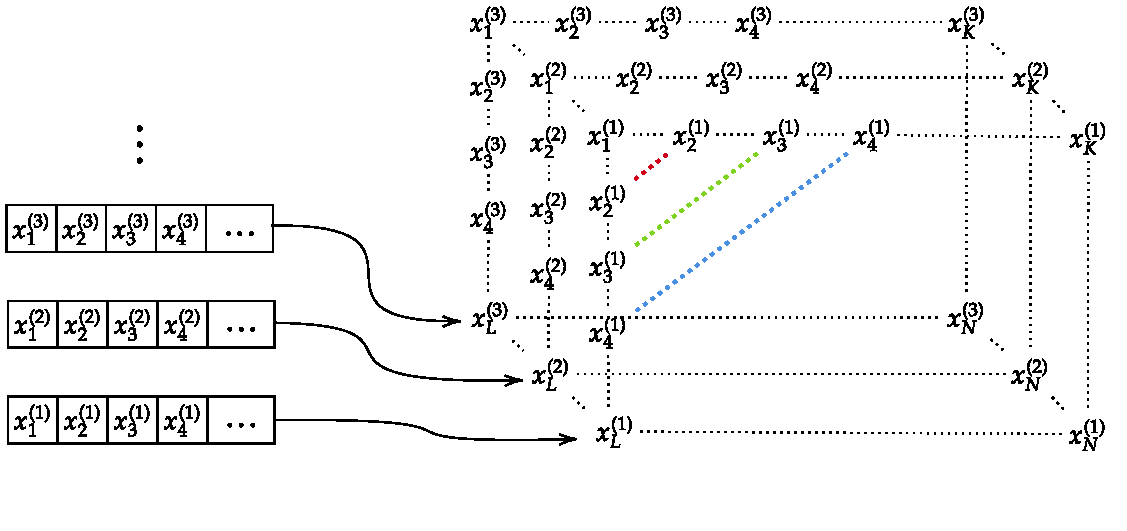
\includegraphics[width=\textwidth]{./img/mssa_injection_new}
    \end{frame}
    
    \begin{frame}{HOSVD-MSSA для разделения компонент сигнала}
        Пусть $\tX = \sum_{m=1}^{M} \tX_m + \tE$ --- $P$-мерный временной ряд\\ \vspace{0.2cm}
        
        \bluetext{Параметры алгоритма:} $L$ --- длина окна, $K=N-L+1$\\{}
        $R$, $\gI_1,\ldots, \gI_M$ --- как в MSSA\\
        $R_3$ --- число элементов разложения по третьему направлению\\
        $\gP_1,\ldots, \gP_M \subseteq \{1,2,\ldots R_3\}$, $\gP_i \cap \gP_j = \varnothing$ --- индексы группировки по 
        третьему направлению
        \begin{itemize}
            \item \bluetext{Вложение} $\tX \overset{L}{\longmapsto} \calX$ --- траекторный тензор\item \bluetext{Разложение} 
            \[
                \calX = \sum_{l=1}^{d_1}\sum_{k=1}^{d_2}
                \sum_{p=1}^{d_3} \calZ_{lkp} U^{(1)}_l \circ U^{(2)}_k \circ U^{(3)}_p
            \]
            \item \bluetext{Группировка} 
            \[
                \widetilde{\calX}_m = \sum_{l\in \gI_m} \sum_{k\in \gI_m} \sum_{p\in \gP_m}
                \calZ_{lkp} \bfU_l^{(1)} \circ \bfU_k^{(2)} \circ \bfU_p^{(3)} 
            \]
            \item \bluetext{Восстановление} усреднение сечений третьего направления $\widetilde{\calX}_m$
             по побочным диагоналям
        \end{itemize}
        
        \vspace{0.2cm}
        
        \bluetext{Результат алгоритма:} $\widetilde{\tX}_m$ --- оценка $\tX_m$
    \end{frame}
    
    
    \section{Свойства HOSVD-MSSA}\label{sec:hosvd-mssa-properties}
    \begin{frame}{Ранг сигнала в HOSVD-MSSA}
        \begin{theorem}
            Пусть $\tX$ --- $P$-мерный временной ряд длины $N$, тогда справедливы следующие утверждения.
            \begin{enumerate}
                \item $\tX$ имеет ранг $d$ в терминах теории \textup{MSSA} тогда и только тогда, когда для траекторного тензора $\calX$, построенного по любой длине окна $L<N$ такой, что 
                $d \leqslant\min(L, K)$ выполняется 
                \[\operatorname{rank}_1(\calX) = \operatorname{rank}_2(\calX) = d.\]
                \item $\operatorname{rank}_3(\calX)$ равен рангу матрицы, 
                в строках которой содержатся одномерные временные ряды, составляющие заданный 
                многомерный ряд.
            \end{enumerate}
        \end{theorem}
    \end{frame}
    
    \begin{frame}{Разделимость в HOSVD-MSSA}
        $\widehat{\tX}$, $\widetilde{\tX}$, $\tX$ --- многомерные временные ряды, $\tX = \widehat{\tX} + \widetilde{\tX}$\\ \vspace{0.1cm}
        $\widehat{\calX}$, $\widetilde{\calX}$, $\calX$ --- траекторные тензоры рядов 
        $\widehat{\tX}$, $\widetilde{\tX}$, $\tX$ с длиной
        окна $L$\\ \vspace{0.2cm}
        $\Lambda_I(\tX) = \operatorname{span}\left\{\left(x_i^{(p)}, x_{i+1}^{(p)}, \ldots, x_{i + I - 1}^{(p)}\right)\right\}$
        \begin{theorem}
            Такие HOSVD тензоров $\widehat{\calX}$ и $\widetilde{\calX}$, что их сумма является HOSVD тензора $\calX$
            существуют тогда и только тогда, когда
            $\Lambda_L(\widehat{\tX}) \perp \Lambda_L(\widetilde{\tX})$ и $\Lambda_K(\widehat{\tX})\perp\Lambda_K(\widetilde{\tX})$
        \end{theorem}
        \vspace{0.2cm}
        \begin{itemize}
            \item Строже, чем для MSSA!
        \end{itemize}
    \end{frame}
    
    
    \section{Численные сравнения}\label{sec:numerical-comparison}
    \begin{frame}{Численные сравнения в задаче разделения компонент}
        \begin{gather*}
            \tX = \left(\tX_1: \tX_2: \ldots: \tX_P\right),\\
            \tX_p = \left(x_1^{(p)}, x_2^{(p)}, \ldots, x_N^{(p)}\right)^{\rmT},\\
            x_n^{(p)} = \hat{s}_n^{(p)} + \tilde{s}_n^{(p)} + \varepsilon_n^{(p)},
        \end{gather*}
        $\varepsilon_n^{(p)}$ --- независимые случайные величины с распределением $\rmN(0, 0.01)$\\ \vspace{0.2cm}
        Оценка точности --- среднеквадратичное отклонение (RMSE):
        \[
             \text{RMSE} = \sqrt{\frac{1}{m} \sum_{i=1}^{m} \text{MSE}\left(\tS, \widetilde{\tS}_i\right)},
             \quad \text{MSE}\left(\tS, \widetilde{\tS} \right) = \frac{1}{N} \sum_{j=1}^{N}
             \left(s_j - \tilde{s}_j\right)^2,
        \]
    \end{frame}
    
    \begin{frame}{Варианты сигналов}
        \begin{enumerate}
            \item \textbf{Равные по каналам сигналы:} $N = 44$, $P = 12$,
            \begin{equation*}
                \hat{s}_n^{(p)} = 2 \cos(2 \pi n / 5), \quad \tilde{s}_n^{(p)} = \cos(2\pi n /3)
            \end{equation*}
            \item \textbf{Различные по каналам амплитуды:} $N = 44$, $P = 12$,
            \begin{gather*}
                \hat{s}_n^{(p)} = 2 c_1^{(p)} \cos(2 \pi n / 5), \quad \tilde{s}_n^{(p)} = c_2^{(p)}\cos(2\pi n /3)
            \end{gather*}
            \item \textbf{Линейные по каналам фазы:} $N = 44$, $P = 12$,
            \begin{equation*}
                \hat{s}_n^{(p)} = 2 c_1^{(p)} \cos(2 \pi n / 5 + p \pi / 6),
                \quad \tilde{s}_n^{(p)} = c_2^{(p)}\cos(2\pi n /3 + p \pi / 9)
            \end{equation*}
            \item \textbf{Произвольные фазы сигналов:} $N = 44$, $P = 12$,
            \begin{gather*}
                \hat{s}_n^{(p)} = 2 c_1^{(p)} \cos(2 \pi n / 5 + \varphi_1^{(p)}),
                \quad \tilde{s}_n^{(p)} = c_2^{(p)}\cos(2\pi n /3 + \varphi_2^{(p)})
            \end{gather*}
            \item \textbf{Разделимость константы от гармоники:} $N = 44$, $P = 12$,
            \begin{equation*}
                \hat{s}_n^{(p)} = 3 c_1^{(p)},
                \quad \tilde{s}_n^{(p)} = c_2^{(p)}\cos(2\pi n /3)
            \end{equation*}
            \item \textbf{Различные по каналам частоты:} $N = 59$, $P = 12$,
            \begin{gather*}
                \hat{s}_n^{(p)} = 2 \cos(2 \pi n / 5), \quad
                \tilde{s}_n^{(p)} = \begin{cases}
                    \cos(2\pi n /3), & 1 \leqslant p \leqslant 10,\\
                    0.4 \cos(2 \pi n / 6), & 11 \leqslant p \leqslant 12.
                \end{cases}
            \end{gather*}
            \item \textbf{Ортогональность по направлению каналов:} $N = 29$, $P = 12$,
            \begin{gather*}
                \hat{s}_n^{(p)} = 2 \cos(2 \pi n / 5) \cos(2 \pi p / 3), \quad
                \tilde{s}_n^{(p)} = 0.5 \cos(2\pi n /3) \cos(2 \pi p / 6)
            \end{gather*}
        \end{enumerate}
    \end{frame}
    \begin{frame}{Среднеквадратичные отклонения оценок компонент}
        \begin{table}[!h]
            \centering
            \begin{tabular}{l|ccc}
                \hline
                Вид сигнала    & MSSA & HOSVD-MSSA    & 2D-SSA \\
                \hline
                Равные сигналы & \begin{tabular}{c} 0.026 \\ \hline 0.025 \end{tabular} &
                \begin{tabular}{c} 0.019 \\ \hline 0.016 \end{tabular}    &
                \begin{tabular}{c} \textbf{0.014} \\ \hline \textbf{0.014} \end{tabular}   \\
                \hline
                Различие амплитуд & \begin{tabular}{c} 0.029 \\ \hline 0.029 \end{tabular} &
                \begin{tabular}{c} \textbf{0.019} \\ \hline \textbf{0.019} \end{tabular}    &
                \begin{tabular}{c} 0.086 \\ \hline 0.083 \end{tabular}   \\
                \hline
                Линейные фазы & \begin{tabular}{c} \textbf{0.026} \\ \hline \textbf{0.025} \end{tabular} &
                \begin{tabular}{c} \textbf{0.025} \\ \hline \textbf{0.025} \end{tabular}    &
                \begin{tabular}{c} 0.117 \\ \hline 0.114 \end{tabular}   \\
                \hline
                Произвольные фазы & \begin{tabular}{c} \textbf{0.026} \\ \hline \textbf{0.025} \end{tabular} &
                \begin{tabular}{c} \textbf{0.025} \\ \hline \textbf{0.025} \end{tabular}    &
                \begin{tabular}{c} 0.034 \\ \hline 0.033 \end{tabular}   \\
                \hline
                Разделимость с $\operatorname{const}$ & \begin{tabular}{c} \textbf{0.017} \\ \hline 0.025 \end{tabular}
                &
                \begin{tabular}{c} \textbf{0.017} \\ \hline \textbf{0.019} \end{tabular}    &
                \begin{tabular}{c} 0.023 \\ \hline 0.033 \end{tabular}   \\
                \hline
                Различие частот & \begin{tabular}{c} 0.024 \\ \hline 0.024 \\ \hline 0.024 \end{tabular} &
                \begin{tabular}{c} 0.018 \\ \hline \textbf{0.018} \\ \hline \textbf{0.014} \end{tabular}    &
                \begin{tabular}{c} \textbf{0.012} \\ \hline 0.031 \\ \hline 0.026 \end{tabular}   \\
                \hline
                \hspace{-0.32cm}
                \begin{tabular}{l}Ортогональность\\ по каналам \end{tabular} & 
                \begin{tabular}{c} 0.031 \\ \hline 0.030 \end{tabular} &
                \begin{tabular}{c} \textbf{0.023} \\ \hline \textbf{0.022} \end{tabular}    &
                \begin{tabular}{c} 0.025 \\ \hline 0.024 \end{tabular}   \\
                \hline
            \end{tabular}\label{tab:comparison-sep-rmse}
        \end{table}
    \end{frame}
    
%    \begin{frame}{Имеющиеся результаты}
%        Работы, в котрых предлагается использовать тензорные разложения в задачах
%        выделения сигнала из ряда:
%        \begin{enumerate}
%            \item Papy, De~Lathauwer et al. (2005), Exponential data fitting using
%            multilinear algebra: the single-channel and multi-channel case
%            \item Kouchaki, Sanei (2013), Tensor based singular spectrum analysis for
%            nonstationary source separation
%            \item Yang et al. (2017), Improved tensor-based Singular Spectrum Analysis
%            based on single channel blind source separation algorithm and its application
%            to fault diagnosis
%        \end{enumerate}
%        \vspace{0.2cm}
%        
%        В работе~1 рассматривается задача оценки параметров одномерных и многомерных
%        сигналов особого вида с использованием тензорного разложения HOSVD.\\
%        В работах 2 и 3 --- задача выделения сигнала из временного ряда с использованием
%        тензорного разложения CPD.
%    \end{frame}
%    
%%    \section{Тензорные модификации алгоритмов}
%    \begin{frame}{ESPRIT}
%        $\tX = (x_1, x_2, \ldots, x_N) = \tS + \tR$, $L$ -- длина окна,\\
%        $K = N - L + 1 \geqslant L$.\\
%        \vspace{0.1cm}
%        
%        \bluetext{Модель:} $s_n = \sum_{j=1}^{r} a_j \exp \{i \varphi_j\} 
%        \exp \{(-\alpha_j + 2 \pi i \omega_j) n\}$\\
%        \bluetext{Параметры алгоритма:} $L$, $R$: $R \leqslant L < N$\\
%        $R$ --- число компонент, относимых к сигналу\\
%        \vspace{0.1cm}
%        
%        \bluetext{Схема алгоритма ESPRIT для оценки $\alpha_j$, $\omega_j$}
%        \begin{enumerate}
%            \item \bluetext{Вложение} $\tX \mapsto \bfX = [X_1 : X_2 : \ldots : X_K] \in \bbR^{L \times K}$,\\
%            $X_i = (x_i, x_{i+1}, \ldots, x_{i+L-1})^{\rmT}$
%            \item \bluetext{Разложение} $\bfX = \sum_{j=1}^{d} \sqrt{\lambda_j}
%            U_j V_j^{\rmT}$, $d \leqslant L$
%            \item \bluetext{Группировка} $\widehat{\bfU} = [U_1: U_2: \ldots: U_R]$, $R\leqslant d$
%            \item \bluetext{Восстановление} $\bfZ: \widehat{\bfU}^{\uparrow} = \widehat{\bfU}_{\downarrow}\bfZ$,\\
%            $\{z_1, z_2, \ldots, z_R\}$ --- собственные числа $\bfZ$
%        \end{enumerate}
%        \bluetext{Результат алгоритма} $z_j$ --- оценка $\exp \{-\alpha_j + 2\pi i \omega\}$
%    \end{frame}
%    
%    \begin{frame}{SSA для выделения сигнала}
%        $\tX = (x_1, x_2, \ldots, x_N) = \tS + \tR$, $L$ -- длина окна,\\
%        $K = N - L + 1 \geqslant L$.\\
%        \vspace{0.2cm}
%        
%        \bluetext{Параметры алгоритма:} $L$, $R$: $R \leqslant L < N$\\
%        $R$ --- число компонент, относимых к сигналу\\
%        \vspace{0.3cm}
%        
%        \bluetext{Схема алгоритма SSA для выделения сигнала}
%        \begin{enumerate}
%            \item \bluetext{Вложение} $\tX \mapsto \bfX = [X_1 : X_2 : \ldots : X_K] \in \bbR^{L \times K}$,\\
%            $X_i = (x_i, x_{i+1}, \ldots, x_{i+L-1})^{\rmT}$
%            \item \bluetext{Разложение} $\bfX = \sum_{j=1}^{d} \sqrt{\lambda_j}
%            U_j V_j^{\rmT}$, $d \leqslant L$
%            \item \bluetext{Группировка}  $\widetilde{\bfS} = \sum_{j=1}^{R} \sqrt{\lambda_j}
%            U_j V_j^{\rmT}$, $R\leqslant d$
%            \item \bluetext{Восстановление} Матрица $\widetilde{\bfS}$ усредняется вдоль побочных
%            диагоналей: $\tilde{s}_k = \operatorname{mean}\left\{\left(\widetilde{\bfS}_{ij}\right)
%            \middle| i + j - 1 = k\right\}$
%        \end{enumerate}
%        \bluetext{Результат алгоритма} $\widetilde{\tS} = (\tilde{s}_1, \tilde{s}_2, \ldots,
%        \tilde{s}_N)$ --- оценка сигнала $\tS$
%    \end{frame}
%    
%    
%    \section{High-Order SSA}\label{sec:known}
%    \begin{frame}{Описание HOSVD}
%        Пусть имеется тензор $\mathcal{A}\in \mathbb{C}^{I_1\times I_2 \times \ldots \times I_M}$, тогда HOSVD $\mathcal{A}$:
%        
%        \begin{equation*}
%            \mathcal{A}=\sum_{i_1=1}^{I_1} \sum_{i_2=1}^{I_2}\ldots \sum_{i_M=1}^{I_M} \mathcal{Z}_{i_1 i_2 \ldots i_M}
%            U^{(1)}_{i_1} \circ U^{(2)}_{i_2} \circ \ldots\circ U^{(M)}_{i_M},
%        \end{equation*}
%        где
%        \begin{itemize}
%            \item $\mathbf{U}^{(n)}=\left[U^{(n)}_{1}: \ldots: U^{(n)}_{I_n}\right]$ --- унитарные матрицы;
%            \smallskip
%            \item Тензор $\mathcal{Z}\in\mathbb{C}^{I_1\times I_2 \times \ldots \times I_M}$ удовлетворяет свойствам
%            \begin{enumerate}
%                \item полная ортогональность:
%                \[
%                \langle\mathcal Z_{i_n=\alpha},\mathcal Z_{i_n=\beta}\rangle=0 \qquad \alpha\ne\beta,
%                \]
%                \item упорядоченность:
%                \begin{equation*}
%                    \|\mathcal Z_{i_n=1}\|\geqslant\|\mathcal Z_{i_n=2}\| \geqslant \ldots \geqslant\|\mathcal Z_{i_n=I_n}\|.
%                \end{equation*}
%            \end{enumerate}
%        \end{itemize}
%    \end{frame}
%    
%    \begin{frame}{Свойства HOSVD}
%        Все свойства представлены в работе De Lathauwer et al. (2000)
%        \begin{itemize}
%            \item HOSVD --- единственное $M$-ортогональное разложение.
%            \vspace{0.3cm}
%            \item При $M=2$ HOSVD совпадает с SVD\@.
%            \vspace{0.3cm}
%            \item Пусть $\operatorname{rank}_n(\mathcal{A})$ --- размерность
%            пространства векторов измерения $n$ тензора.
%            Если в HOSVD тензора $\mathcal{A}$ $r_n$ --- наибольший индекс такой, что $\|\mathcal{Z}_{i_n=r_n}\|>0$,
%            то $r_n=\operatorname{rank}_n(\mathcal{A})$.
%            \vspace{0.3cm}
%            \item
%            \begin{gather*}
%                \|\mathcal{A}\|^2=\sum_{i=1}^{R_1}\left( \sigma_i^{(1)} \right)^2=\sum_{i=1}^{R_2}\left( \sigma_i^{(2)} \right)^2
%                =\ldots =\sum_{i=1}^{R_M}\left( \sigma_i^{(M)} \right)^2= \|\mathcal{Z}\|^2\\
%                \sigma_{i}^{(n)}=\|\mathcal{Z}_{{i_n}=i}\|, \qquad R_n=\operatorname{rank}_n(\mathcal{A}).
%            \end{gather*}
%        \end{itemize}
%    \end{frame}
%    
%    \begin{frame}{Свойства HOSVD}
%        \begin{itemize}
%            \item Векторы тензора $\mathcal{A}$ по измерению $n$ в содержат наибольшие вклады в направлении $U^{(n)}_1$,
%            величина этого вклада равна $\sigma^{(n)^2}_1$.
%            Следующий по величине вклад по измерению $n$ достигается в направлении $U^{(n)}_2$,
%            перпендикулярном $U^{(n)}_1$, с величиной $\sigma^{(n)^2}_2$, и т.д.
%            \vspace{0.4cm}
%            \item Определим тензор $\hat{\mathcal{A}}$ обнулением наименьших сингулярных значений $\sigma_{I_{n}'+1}^{(n)},
%            \sigma_{I_{n}'+2}^{(n)},\ldots, \sigma_{R_n}^{(n)}$, тогда
%            \begin{equation*}
%                \|\mathcal{A}-\hat{\mathcal{A}}\|^2\leqslant \sum_{i_1=I_{1}'+1}^{R_1}\left( \sigma_{i_1}^{(1)}\right)^2 +
%                \ldots + \sum_{i_M=I_{M}'+1}^{R_M}\left( \sigma_{i_M}^{(M)}\right)^2.
%            \end{equation*}
%        \end{itemize}
%    \end{frame}
%    
%    
%    \section{HOSVD SSA: выделение сигнала}\label{sec:tssa-intro}
%    
%    \begin{frame}{Построение тензора}
%        \centering
%        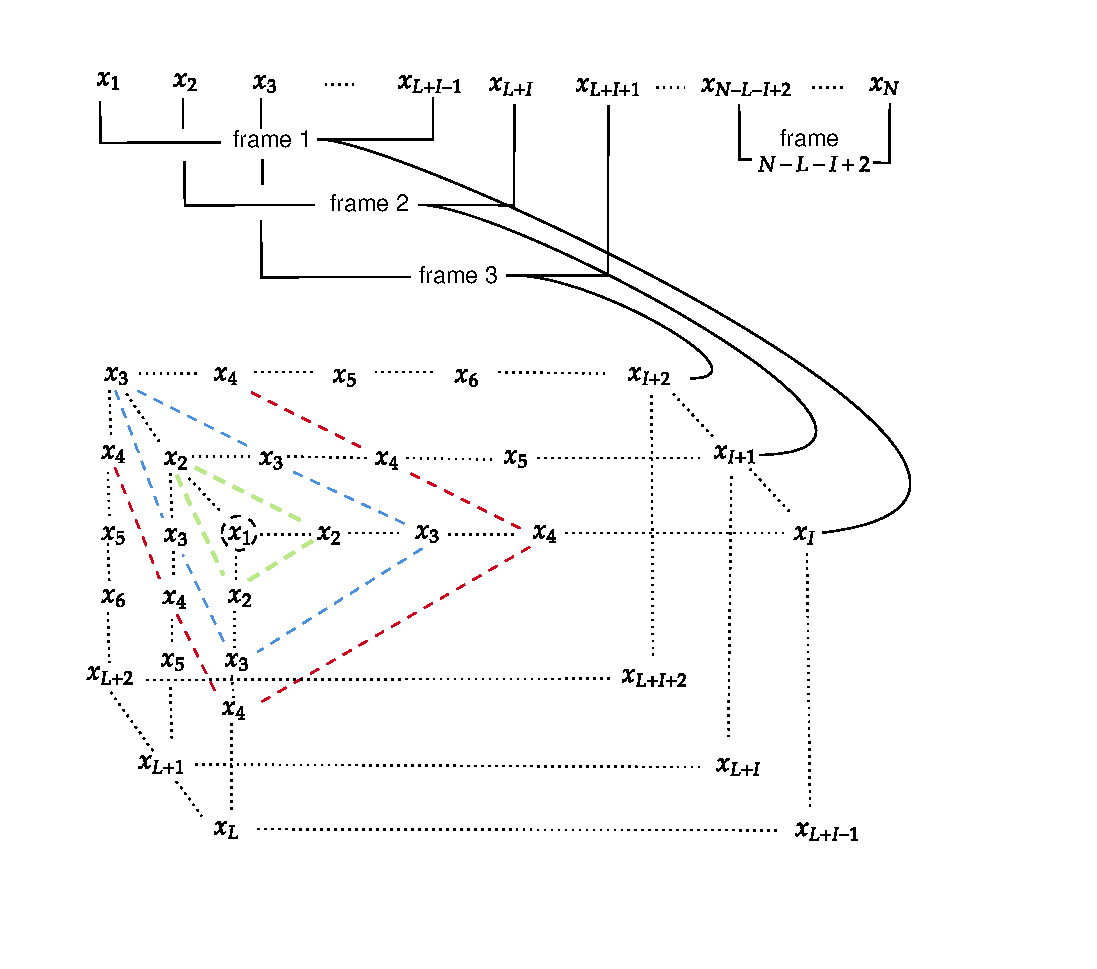
\includegraphics[width = \textwidth, height=0.8\textheight]{./img/tensor_injection_diagram}\\
%        $I, L$ --- параметры длины окна
%    \end{frame}
%    
%    \begin{frame}{High-Order SSA для выделения сигнала}
%        \begin{itemize}
%            \item \bluetext{n-ранг тензора:} размерность пространства, порождённого векторами вдоль
%            $n$-измерения тензора
%            \item В отличие от матричного случая, $n$-ранги тензора произвольной размерности могут в общем случае
%            не совпадать
%        \end{itemize}
%        
%        \vspace{0.4cm}
%        
%        Основная идея алгоритма выделения сигнала --- приблизить траекторный тензор тензором с фиксированными
%        $n$-рангами, меньшими, чем у исходного.
%    \end{frame}
%    
%    \begin{frame}{HOSVD SSA: разложение и группировка}
%        \begin{itemize}
%            \item \bluetext{Разложение:} HOSVD траекторного тензора $\calX$ имеет вид
%            \[
%            \mathcal{X}=\sum_{i=1}^{I} \sum_{l=1}^{L} \sum_{j=1}^{N - I - L + 2} \mathcal{Z}_{ilj} \mathbf{U}^{(1)}_{i}
%            \circ \mathbf{U}^{(2)}_{l} \circ \mathbf{U}^{(3)}_{j}
%            \]
%            
%            \vspace{0.2cm}
%            \item \bluetext{Группировка:}
%            \[
%            \widetilde{\calX} =\sum_{i=1}^{R} \sum_{l=1}^{R} \sum_{j=1}^{R} \mathcal{Z}_{ilj} \mathbf{U}^{(1)}_{i}
%            \circ \mathbf{U}^{(2)}_{l} \circ \mathbf{U}^{(3)}_{j}
%            \]
%            $R \leqslant \min(I, L, N-I-L+2)$ --- параметр алгоритма
%            
%            \vspace{0.2cm}
%            \item \bluetext{Восстановление:} усреднение тензора $\widetilde{\calX}$ вдоль побочных плоскостей
%            $\left\{i + l + j = \operatorname{const}\right\}$
%        \end{itemize}
%    \end{frame}
%    
%    \section{HOOI SSA}
%    \begin{frame}{Higher Order Orthogonal Iteration (HOOI)}
%        Другой метод приближения произвольного тензора тензором заданных $n$-рангов --- Higher Order Orthogonal Iteration (HOOI).\\
%        Описание алгоритма HOOI и его свойства приведены в работе Sheehan et al. (2007) Higher Order Orthogonal Iteration of Tensors (HOOI) and its Relation to PCA and GLRAM.\\
%        При заданных $\calA \in \bbR^{I_1 \times I_2 \times \ldots \times I_M}$ и ($R_1, R_2, \ldots, R_M$)
%        минимизируется норма Фробениуса 
%        \[
%        \| \calA - \widetilde{\calA}\|^2 \to \min,
%        \]
%        где $\min$ по всем $\widetilde{\calA}: \widetilde{\calA} \in \bbR^{I_1 \times I_2 \times \ldots \times I_M}$, 
%        $\operatorname{rank}_n(\widetilde{\calA}) = R_i$
%    \end{frame}
%    
%    \begin{frame}{HOOI SSA: разложение и восстановление}
%        \begin{itemize}
%            \item \bluetext{HOOI:} Выбор ранга сигнала $r$ и применение к траекторному тензору $\calX$ HOOI c 
%            набором $n$-рангов $(r,r,r)$. Результат --- оптимальное приближение тензором $\widehat{\calX}$ с 
%            $n$-рангами $r$
%            \item \bluetext{Восстановление:} усреднение тензора $\widehat{\calX}$ аналогично восстановлению в 
%            варианте с усечением HOSVD
%        \end{itemize}
%        \vspace*{0.4cm}
%        
%        \bluetext{Результат алгоритма:} полученный усреднением ряд $\widehat{\tX}$ --- оценка сигнала $\tS$
%    \end{frame}
%    
%    \section{Свойства HO-SSA в задаче выделения сигнала}
%    \begin{frame}{Ранг сигнала}
%        $\tS$ имеет ранг $r$, если $r < N / 2$ и \\
%        $\forall L: r \leqslant \min(L, K)\quad \operatorname{rank}\bfS = r$\\
%        \vspace{0.2cm}
%        
%        Рекомендуемый выбор параметра $R$ в алгоритме: $R = r$\\
%        \vspace{0.4cm}
%        
%        \bluetext{Примеры}
%        \begin{enumerate}
%            \item $s_n = \cos(2 \pi n \omega + \psi), \qquad n \in \overline{1:N}$,\\
%            $0 < \omega < 1/2$, $\psi \in [0, 2\pi)$\\
%            $r = 2$
%            
%            \vspace{0.2cm}
%            
%            \item $s_n = a^n,\qquad n \in \overline{1:N}, \qquad a \ne 0$\\
%            $r =1$
%        \end{enumerate}
%    \end{frame}
%    
%    \begin{frame}{Ранг в HOSVD SSA}
%        \begin{theorem}
%            Пусть сигнал $\tS$ имеет конечный ранг $r$ в терминах \emph{SSA}.\\
%            Тогда для любых значений параметров $I$ и $L$ таких, что
%            \[
%            r \leqslant \min(I, L, N-I-L+2),
%            \] 
%            все $n$-ранги траекторного тензора $\calX$ этого сигнала с длинами окна $I$ и $L$ будут равны $r$.
%        \end{theorem}
%    \end{frame}
%    
%    \begin{frame}{Трудоёмкость алгоритмов HO-SSA}
%        \begin{itemize}
%            \item \bluetext{HOSVD-SSA:} вычисление HOSVD тензора размерности $I\times L \times J$ имеет трудоёмкость порядка
%            \[
%            O(ILJ(\min(I, LJ) + \min(L, IJ) + \min(J, IL))).
%            \]
%            Если требуется вычислить только усечение HOSVD с $n$-рангами $(r_1, r_2, r_3)$, то трудоёмкость можно
%            уменьшить до порядка
%            \[
%            O(ILJ(r_1 + r_2 + r_3)).
%            \]
%            \item \bluetext{HOOI-SSA:} HOOI --- итеративный алгоритм. Трудоёмкость каждой итерации имеет порядок
%            \[
%            O(r_1 r_2 r_3 (I + L + J)),
%            \]
%            а скорость сходимости алгоритма линейная.
%        \end{itemize} 
%    \end{frame}
%    
%    \section{HOSVD-SSA: разделение компонент сигнала}
%    \begin{frame}{HOSVD SSA: разделение компонент сигнала}
%        Пусть $\tS = \sum_{k=1}^{m} \tS_k$\\
%        Шаги вложения и разложения совпадают с алгоритмом HOSVD SSA для выделения сигнала.
%        \begin{itemize}
%            \item \bluetext{Группировка:} разбиение множества индексов $\mathfrak{S}=\{1,\, 2\,\ldots,\, \min(I, L, J)\}$ по смыслу на
%            непересекающиеся множества $\mathfrak{S}_k,\, k\in\overline{1:m}$ и построение по этому разбиению тензоров
%            \[
%            \mathcal{X}^{(\mathfrak{S}_k)}=\sum_{i \in \mathfrak{S}_k} \sum_{l\in \mathfrak{S}_k} \sum_{j\in \mathfrak{S}_k}
%            \mathcal{Z}_{ilj} \mathbf{U}^{(1)}_{i}\circ \mathbf{U}^{(2)}_{l} \circ \mathbf{U}^{(3)}_{j}.
%            \]
%            \item \bluetext{Восстановление:} получение рядов $\widetilde{\tS}_k$ по тензорам
%            $\mathcal{X}^{(\mathfrak{S}_k)}$ посредством их усреднения вдоль плоскостей
%            ${\{i+l+j=\operatorname{const}\}}$
%        \end{itemize}
%        
%        \vspace{0.1cm}
%        \bluetext{Результат алгоритма:} $\widetilde{\tS}_k$ --- оценка $\tS_k$.
%    \end{frame}
%    
%    \begin{frame}{Разделимость рядов в HOSVD-SSA}
%        \bluetext{Разделимость} рядов является важным понятием в теории SSA
%        
%        \vspace{0.5cm}
%        \begin{theorem}
%            Временные ряды $\widetilde{\tX}$ и $\widehat{\tX}$ длины $N$ слабо $I$- и
%            $L$-разделимы в смысле теории \emph{SSA} тогда и только тогда, когда существует такое 
%            \emph{HOSVD} траекторного тензора $\mathcal{X}$ ряда
%            $\tX=\widetilde{\tX} + \widehat{\tX}$, что его можно в виде суммы \emph{HOSVD} траекторных тензоров рядов
%            $\widetilde{\tX}$ и $\widehat{\tX}$.
%        \end{theorem}
%        
%        \vspace{0.6cm}
%        Понятие слабой разделимости рядов из SSA применимо к HO-SSA
%    \end{frame}
%    
%    
%    \section{HOSVD-MSSA}
%    \begin{frame}{MSSA}
%        \bluetext{Многомерный временной ряд:}\\
%        $\tX = \left(\tX_1: \tX_2: \ldots: \tX_P\right), \qquad \tX_p = \left(x_1^{(p)}, x_2^{(p)}, \ldots, x_N^{(p)}\right)^{\rmT}$\\
%        \vspace{0.2cm}
%        
%        \bluetext{Траекторная матрица этого ряда:}\\
%        $\bfX = \left[\bfX_1 : \bfX_2 : \ldots : \bfX_P\right]$,\\
%        $\bfX_p$ --- траекторная матрица $\tX_p$\\
%        \vspace{0.2cm}
%        
%        Дальнейшие шаги алгоритма MSSA (разложение траекторной матрицы и восстановление сигнала) аналогичны
%        стандартному SSA.\\
%        \vspace{0.2cm}
%        
%        В случаях, когда сигналы $\tS_p$ имеют похожую структуру, использование MSSA даёт лучшие результаты, чем
%        применение SSA к каждому ряду отдельно.
%    \end{frame}
%    
%    \begin{frame}{HOSVD-MSSA}
%        Вместо матрицы $\bfX = \left[\bfX_1:\bfX_2 :\ldots: \bfX_P\right]$\\
%        строится тензор $\calX: \calX_{\cdot \cdot p} = \bfX_p$
%        
%        \centering
%        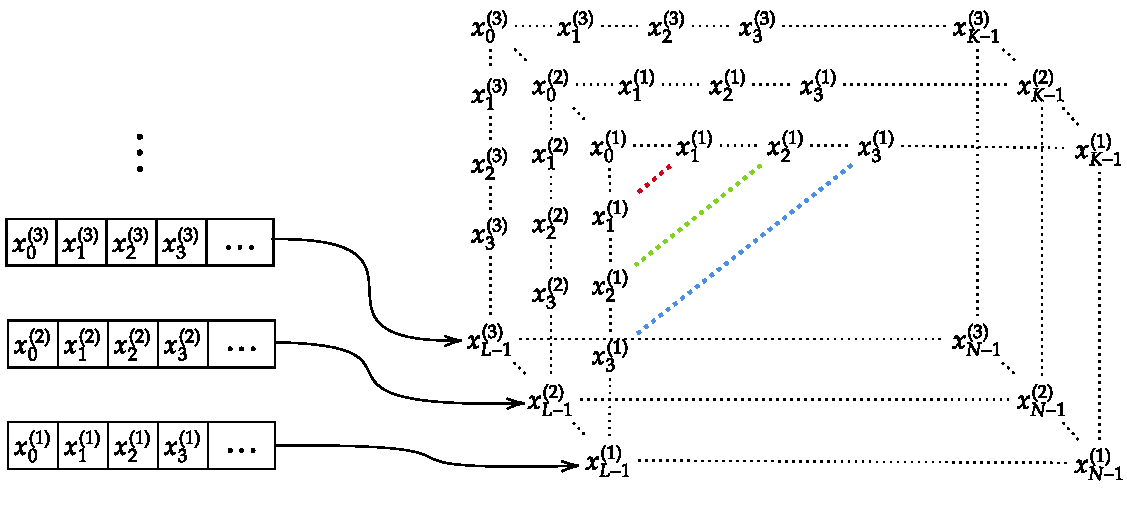
\includegraphics[width=\textwidth]{./img/mssa_injection}
%    \end{frame}
%    
%    \section{Свойства HOSVD-MSSA для выделения сигнала}
%    \begin{frame}{Ранг сигнала в HOSVD-MSSA}
%        \begin{theorem}
%            Пусть $\tX$ --- $P$-мерный временной ряд длины $N$, тогда справедливы следующие утверждения.
%            \begin{enumerate}
%                \item $\tX$ имеет ранг $d$ в терминах теории \emph{MSSA} тогда и только тогда, когда для траекторного тензора $\calX$, построенного по любой длине окна $L<N$ такой, что 
%                $d \leqslant\min(L, K)$ выполняется 
%                \[\operatorname{rank}_1(\calX) = \operatorname{rank}_2(\calX) = d.\]
%                \item 3-Ранг $\calX$ равен рангу матрицы, 
%                в строках которой содержатся одномерные временные ряды, составляющие заданный 
%                многомерный ряд.
%            \end{enumerate}
%        \end{theorem}
%    \end{frame}
%    
%    
%    \begin{frame}{Ранг сигнала в HOSVD-MSSA}
%        \begin{itemize}
%            \item 1- и 2-ранги траекторного тензора $\calX$ сигнала $\tS$ совпадают с рангом этого сигнала в терминах
%            MSSA
%            \item 3-ранг имеет смысл степени структурного различия одномерных сигналов, составляющих данный многомерный
%        \end{itemize}
%        
%        \vspace*{0.2cm}
%        
%        На этапе группировки рекомендуется брать $R_1=R_2=r$ и $R_3=r_3$, где $r$ --- MSSA-ранг сигнала, а 
%        $r_3$ --- ранг матрицы, составленной из $\tS_p$\\
%        \vspace{0.3cm}
%        
%        \bluetext{Примеры}
%        $s_n^{(p)} = a_p \cos(2 \pi n \omega_p + \psi_p),\, p\in \{1, 2\},\, n \in \overline{1:N}$,\\
%        $a_p \ne 0,\, 0 < \omega_p < 1/2,\, \psi_p \in [0, 2\pi)$
%        \begin{enumerate}
%            \item $\psi_1 = \psi_2,\, \omega_1 = \omega_2 \implies r = r_1 = r_2 = 2,\, r_3 = 1$ 
%            \item $\psi_1 \ne \psi_2,\, \omega_1 = \omega_2 \implies r = r_1 = r_2 = 2,\, r_3 = 2$ 
%            \item \hspace{42pt} $\omega_1 \ne \omega_2 \implies r = r_1 = r_2 = 4,\, r_3 = 2$ 
%        \end{enumerate}
%    \end{frame}
%    
%    \section{HO-MSSA: разделение компонент сигнала}
%    \begin{frame}{HO-MSSA: разделение компонент сигнала}
%        Пусть $\tS = \sum_{m=1}^{M} \tS_m$\\
%        Шаги вложения и разложения совпадают с алгоритмом HO-MSSA для выделения сигнала
%        
%        \begin{itemize}
%            \item \bluetext{Группировка} разбиение множества индексов ${\gS = \{1, 2, \ldots, \min(L, K)\}}$ и
%            $\gP = \{1, 2, \ldots, P\}$ по смыслу
%            на подмножества $\gS_m$ и $\gP_m$, $m \in \overline{1:M}$, и построение по этому разбиению 
%            тензоров
%            \[
%            \calX_m = \sum_{l\in \gS_m} \sum_{k\in \gS_m} \sum_{p\in \gP_m}
%            \calZ_{lkp} \bfU_l^{(1)} \circ \bfU_k^{(2)} \circ \bfU_p^{(3)} 
%            \]
%            \item \bluetext{Восстановление} получение рядов $\widetilde{\tS}_m$ по тензорам $\calX_m$ 
%            путём усреднения их слоёв вдоль побочных диагоналей
%        \end{itemize}
%        
%        \vspace{0.2cm}
%        
%        \bluetext{Результат алгоритма:} $\widetilde{\tS}_m$ --- оценка $\tS_m$
%    \end{frame}
%    
%    \begin{frame}{HO-MSSA: разделение компонент сигнала}
%        $\widehat{\tX}$, $\widetilde{\tX}$, $\tX$ --- многомерные временные ряды, $\tX = \widehat{\tX} + \widetilde{\tX}$\\
%        $\widehat{\calX}$, $\widetilde{\calX}$, $\calX$ --- траекторные тензоры рядов 
%        $\widehat{\tX}$, $\widetilde{\tX}$, $\tX$ с длиной
%        окна $L$\\
%        $\Lambda_I(\tX) = \operatorname{span}\left\{(x_i^{(p)}, x_{i+1}^{(p)}, \ldots, x_{i + I - 1}^{(p)})\right\}$
%        \begin{theorem}
%            Такие HOSVD тензоров $\widehat{\tX}$ и $\widetilde{\tX}$, что их сумма является HOSVD тензора $\calX$ существуют
%            тогда и только тогда, когда ортогональны пары пространств: \\
%            $\Lambda_L(\widehat{\tX})$ с $\Lambda_L(\widetilde{\tX})$ и $\Lambda_K(\widehat{\tX})$ с
%            $\Lambda_K(\widetilde{\tX})$
%        \end{theorem}
%        
%        Этот критерий разделимости более строгий, чем в алгоритме MSSA\\
%        \vspace{0.2cm}
%        
%        Этот критерий позволяет вывести рекомендации по выбору параметров $L$, $\gS_m$, $\gP_m$
%    \end{frame}
%    
%    
%    \section{Численные сравнения}
%    \begin{frame}{Численные сравнения: выделение сигнала}
%        \begin{gather*}
%            \tX = \left(\tX_1:\ldots : \tX_P\right),\\
%            \tX_p = \left(s_1^{(p)} + \varepsilon_1^{(p)}, \ldots, s_N^{(p)} + \varepsilon_N^{(p)}\right),\\
%            s_n^{(p)} = a_p \cos(2\pi n \omega_p + \psi_p),
%        \end{gather*}
%        где $n \in \overline{1:71}$, $p\in \overline{1:5}$, $\varepsilon_n^{(p)}$ --- белый гауссовский шум с дисперсией 25,
%        $s_n^{(p)}$ --- элементы искомого сигнала.\\
%        \vspace*{0.2cm}
%        
%        Оценка точности --- RMSE по 500 реализациям шума.
%    \end{frame}
%    
%    \begin{frame}{Численные сравнения: ранги сигналов}
%        
%        \begin{table}
%            \hspace*{-0.4cm}
%            \footnotesize
%            \begin{tabular}{c|cccc}
%                Параметры & (HOOI) SSA & (HOSVD) MSSA & $r_3$ & 2D-SSA \\ \hline
%                \begin{tabular}{c}
%                    $a_p=30$\\
%                    $\omega_p = 1/12,\, \psi_p = 0$
%                \end{tabular} & 2 & 2 & 1 & 2 \\ \hline
%                \begin{tabular}{c}
%                    $a_1 = a_4 = 30$\\
%                    $a_2=a_5=20$, $a_3 = 25$\\
%                    $\omega_p = 1/12,\, \psi_p = 0$
%                \end{tabular} & 2 & 2 & 1 & 6 \\ \hline
%                \begin{tabular}{c}
%                    $a_p=30$, $\omega_p=1/12$ \\
%                    $\psi_p = 2(p-1)\pi / 3$
%                \end{tabular} & 2 & 2 & 2 & 2 \\ \hline
%                \begin{tabular}{c}
%                    $a_p=30$, $\psi_p = 2(p-1)\pi / 3$\\
%                    $\omega_1=\omega_2=\omega_3=1/12$ \\
%                    $\omega_4=\omega_5=1/8$ 
%                \end{tabular} & 2 & 4 & 4 & 10 \\ \hline
%            \end{tabular}
%        \end{table}
%    \end{frame}
%    
%    \begin{frame}{Численные сравнения: RMSE оценок сигналов}
%        
%        \begin{table}
%            \hspace*{-0.6cm}
%            \scriptsize
%            \begin{tabular}{c|ccccc}
%                Параметры & SSA & HOOI-SSA & MSSA & HOSVD-MSSA & 2D-SSA \\ \hline
%                \begin{tabular}{c}
%                    $a_p=30$\\
%                    $\omega_p = 1/12,\, \psi_p = 0$
%                \end{tabular} & 1.34 & 1.41 & 0.95 & 0.75 & \textbf{0.73} \\ \hline
%                \begin{tabular}{c}
%                    $a_1 = a_4 = 30$\\
%                    $a_2=a_5=20$, $a_3 = 25$\\
%                    $\omega_p = 1/12,\, \psi_p = 0$
%                \end{tabular} & 1.38 & 1.41 & 1.07 & \textbf{0.86} & 1.45 \\ \hline
%                \begin{tabular}{c}
%                    $a_p=30$, $\omega_p=1/12$ \\
%                    $\psi_p = 2(p-1)\pi / 3$
%                \end{tabular} & 1.38 & 1.41 & 1.07 & 1.05 & \textbf{0.84} \\ \hline
%                \begin{tabular}{c}
%                    $a_p=30$, $\psi_p = 2(p-1)\pi / 3$\\
%                    $\omega_1=\omega_2=\omega_3=1/12$ \\
%                    $\omega_4=\omega_5=1/8$ 
%                \end{tabular} & \textbf{1.38} & 1.41 & 1.50 & 1.49 & 1.78 \\ \hline
%            \end{tabular}
%        \end{table}
%    \end{frame}
%    
%    \begin{frame}{Численные сравнения: разделимость многомерных рядов}
%        \[
%        x_n^{(p)} = \hat{s}_n^{(p)} + \tilde{s}_n^{(p)} + \varepsilon_n^{(p)}
%        \]
%        \vspace*{0.1cm}
%        
%        $n \in \overline{1:44}$, $p \in \overline{1:12}$
%        
%        Рассматриваемые варианты рядов:
%        \begin{enumerate}
%            \item $\hat{s}_n^{(p)} = 2 \cos(2 \pi n / 5), \quad \tilde{s}_n^{(p)} = \cos(2\pi n /3)$
%            
%            \vspace{0.1cm}
%            
%            \item $\hat{s}_n^{(p)} = 2 c_1^{(p)} \cos(2 \pi n / 5), \quad \tilde{s}_n^{(p)} = c_2^{(p)}\cos(2\pi n /3)$
%            
%            \vspace{0.1cm}
%            
%            \item $\hat{s}_n^{(p)} = 2 c_1^{(p)} \cos(2 \pi n / 5 + p \pi / 6)$, \\
%            $\tilde{s}_n^{(p)} = c_2^{(p)}\cos(2\pi n /3 + p \pi / 9)$
%            
%            \vspace{0.1cm}
%            
%            \item $\hat{s}_n^{(p)} = 2 c_1^{(p)} \cos(2 \pi n / 5 + \varphi_1^{(p)})$,\\ 
%            $\tilde{s}_n^{(p)} = c_2^{(p)}\cos(2\pi n /3 + \varphi_2^{(p)})$
%        \end{enumerate}
%    \end{frame}
%    
%    \begin{frame}{Численные сравнения: разделимость многомерных рядов}
%        
%        \begin{enumerate}
%            \setcounter{enumi}{4}
%            \item $\hat{s}_n^{(p)} = 3 c_1^{(p)}, 
%            \quad \tilde{s}_n^{(p)} = c_2^{(p)}\cos(2\pi n /3)$
%            
%            \vspace{0.2cm}
%            
%            \item $\hat{s}_n^{(p)} = 2 \cos(2 \pi n / 5)$,\\ 
%            $\tilde{s}_n^{(p)} = \begin{cases}
%                \cos(2\pi n /3), & 1 \leqslant p \leqslant 10,\\
%                0.4 \cos(2 \pi n / 6), & 11 \leqslant p \leqslant 12
%            \end{cases}$
%            
%            $n \in \overline{1:59}$
%            
%            \vspace{0.2cm}
%            
%            \item $\hat{s}_n^{(p)} = 2 \cos(2 \pi n / 5) \cos(2 \pi p / 3)$,\\ 
%            $\tilde{s}_n^{(p)} = 0.5 \cos(2\pi n /3) \cos(2 \pi p / 6)$
%        \end{enumerate}
%        
%        \vspace*{0.4cm}
%        
%        $\varepsilon_n^{(p)}$ --- белый гауссовский шум со стандартным отклонением $0.1$\\
%        Оценка точности --- RMSE по 1000 реализациям шума.
%    \end{frame}
%    
%    \begin{frame}{Численные сравнения: RMSE оценок компонент сигнала}
%        
%        \begin{table}
%            \footnotesize
%            \hspace*{-0.3cm}
%            \begin{tabular}{c|ccc}
%                \hline
%                Вид сигнала    & MSSA & HOSVD-MSSA    & 2D-SSA \\
%                \hline
%                1 & \begin{tabular}{c} 0.026 \\ \hline 0.025 \end{tabular} & 
%                \begin{tabular}{c} 0.019 \\ \hline 0.016 \end{tabular}    & 
%                \begin{tabular}{c} \textbf{0.014} \\ \hline \textbf{0.014} \end{tabular}   \\
%                \hhline{-|===}
%                2 & \begin{tabular}{c} 0.029 \\ \hline 0.029 \end{tabular} & 
%                \begin{tabular}{c} \textbf{0.019} \\ \hline \textbf{0.019} \end{tabular}    & 
%                \begin{tabular}{c} 0.086 \\ \hline 0.083 \end{tabular}   \\
%                \hhline{-|===}
%                3 & \begin{tabular}{c} \textbf{0.026} \\ \hline \textbf{0.025} \end{tabular} & 
%                \begin{tabular}{c} \textbf{0.025} \\ \hline \textbf{0.025} \end{tabular}    & 
%                \begin{tabular}{c} 0.117 \\ \hline 0.114 \end{tabular}   \\
%                \hhline{-|===}
%                4 & \begin{tabular}{c} \textbf{0.026} \\ \hline \textbf{0.025} \end{tabular} & 
%                \begin{tabular}{c} \textbf{0.025} \\ \hline \textbf{0.025} \end{tabular}    & 
%                \begin{tabular}{c} 0.034 \\ \hline 0.033 \end{tabular}   \\
%                \hhline{-|===}
%                5 & \begin{tabular}{c} \textbf{0.017} \\ \hline 0.025 \end{tabular} & 
%                \begin{tabular}{c} \textbf{0.017} \\ \hline \textbf{0.019} \end{tabular}    & 
%                \begin{tabular}{c} 0.023 \\ \hline 0.033 \end{tabular}   \\
%                \hhline{-|===}
%                6 & \begin{tabular}{c} 0.024 \\ \hline 0.024 \\ \hline 0.024 \end{tabular} & 
%                \begin{tabular}{c} 0.018 \\ \hline \textbf{0.018} \\ \hline \textbf{0.014} \end{tabular}    & 
%                \begin{tabular}{c} \textbf{0.012} \\ \hline 0.031 \\ \hline 0.026 \end{tabular}   \\
%                \hhline{-|===}
%                7 & \begin{tabular}{c} 0.031 \\ \hline 0.030 \end{tabular} & 
%                \begin{tabular}{c} \textbf{0.023} \\ \hline \textbf{0.022} \end{tabular}    & 
%                \begin{tabular}{c} 0.025 \\ \hline 0.024 \end{tabular}   \\
%                \hline
%            \end{tabular}
%        \end{table}
%    \end{frame}  
%    
%    
%    \section{Заключение}\label{sec:conclusion}
%    \begin{frame}{Выводы}
    %        \begin{itemize}
        %            \item HO-SSA и HOSVD-MSSA являются прямыми обобщениями SSA и MSSA, однако устроены существенно
        %            сложнее и имеют б\'{о}льшую трудоёмкость
        %            \item Обе модификации усложняют алгоритм необходимостью подбора дополнительного параметра
        %            \item В рассмотренных примерах HOSVD-SSA выделил сигнал и разделил компоненты менее точно, чем SSA
        %            \item В рассмотренных примерах HOSVD-MSSA выделил сигнал и разделил компоненты точнее, чем MSSA
        %        \end{itemize}
    %    \end{frame}
%    
%    \begin{frame}{Остаётся для исследования}
    %        \begin{itemize}
        %            \item Возможность применения других тензорных разложений
        %            \item Нахождение семейства сигналов, для которых HOSVD-MSSA работает существенно точнее, чем MSSA и 2D-SSA 
        %            \item Формулировка понятия сильной разделимости для тензорных алгоритмов по аналогии с теорией SSA
        %        \end{itemize}
    %    \end{frame}  
\end{document}
